\chapter*{\hfill APÊNDICE A\hfill}
\addcontentsline{toc}{chapter}{APÊNDICE A}
\renewcommand{\thetable}{A.\arabic{table}}
\renewcommand{\thefigure}{A.\arabic{figure}}
\renewcommand{\theequation}{A.\arabic{equation}}

\noindent\textbf{Exemplo de Cálculo Manual da Equação de Chuvas Intensas}\bigskip

Nesta seção, será apresentado um exemplo de cálculo da equação IDF, para um melhor entendimento das equações explicadas no referencial teórico. Primeiramente são definidos os dados de precipitação diária anual máxima na Tabela A.1, que serão usados nos cálculos e em diante todo o processo de cálculo se seguirá.\bigskip

% Tabela de Precipitações Máximas
\begin{table}[ht]
\centering
\caption{Simulação de \\ Precipitação Máxima Diária Anual.}
\begin{tabular}{
>{\columncolor[HTML]{FFFFFF}}c
>{\columncolor[HTML]{FFFFFF}}c }
\hline
\cellcolor[HTML]{FFFFFF} & \cellcolor[HTML]{FFFFFF} \\
\multirow{-2}{*}{\cellcolor[HTML]{FFFFFF}N} & \multirow{-2}{*}{\cellcolor[HTML]{FFFFFF}Xi} \\ \hline
1969 & 56.5 \\
1986 & 51.8 \\
1970 & 46.0 \\
1975 & 45.2 \\
1977 & 41.0 \\
1978 & 40.2 \\
1968 & 39.7 \\
1987 & 38.6 \\
1981 & 36.9 \\
1976 & 36.8 \\
1982 & 34.5 \\
1979 & 33.7 \\
1971 & 33.6 \\
1980 & 33.4 \\
1974 & 31.7 \\
1973 & 29.9 \\
1972 & 28.0 \\
1985 & 27.6 \\
1983 & 26.4 \\
1984 & 25.0 \\ \hline
\end{tabular}
\caption*{\textbf{Fonte:} De autoria própria (2023).}
\end{table}

Inicia-se então o método de distribuição de Gumbel. Assim sendo tem-se a média em (A.1), a partir da fórmula (3.3) e dos dados da Tabela A.1:\bigskip

% Média das Precipitações Máximas
\begin{equation}
\bar{X} = \frac{736.5}{20} = 36.825 mm
\end{equation}\bigskip

\newpage
 
Desvio padrão (A.2), a partir da fórmula (3.4), Tabela A.1 e média obtida em (A.1):\bigskip

% Desvio Padrão
\begin{equation}
\delta = \sqrt{\frac{1328.938}{20 - 1}} = 8.363
\end{equation}\bigskip

Parâmetro de escala da distribuição de Gumbel (A.3), a partir da fórmula (3.5) e do desvio padrão obtido em (A.2):\bigskip

% Parâmetro Beta de Gumbel
\begin{equation}
\beta_1 = \frac{2.449}{\pi} * 8.363 = 6.521
\end{equation}\bigskip

Moda de Gumbel (A.4), a partir da fórmula (3.6), da média obtida em (A.1) e do parâmetro de escala da distribuição de Gumbel obtido em (A.3):\bigskip

% Moda de Gumbel
\begin{equation}
\mu = 36.825 - \gamma * 6.521 = 33.061 mm
\end{equation}\bigskip

Mediana de Gumbel (A.5) à (A.11), a partir da fórmula (3.7), do parâmetro de escala da distribuição de Gumbel obtido em (A.3), da moda de Gumbel obtida em (A.4), e dos tempos de retorno arbitrados, que para esse exemplo serão de 2, 5, 10, 25, 50, 75 e 100:\bigskip

% Mediana de Gumbel (Precipitação de 24 Horas sem Majoração)
\begin{equation}
Xt = 33.061 - 6.521 * \ln{\left(\ln{\left(\frac{2}{2 - 1}\right)}\right)} = 35.451 mm
\end{equation}

\begin{equation}
Xt = 33.061 - 6.521 * \ln{\left(\ln{\left(\frac{5}{5 - 1}\right)}\right)} = 42.842 mm
\end{equation}

\begin{equation}
Xt = 33.061 - 6.521 * \ln{\left(\ln{\left(\frac{10}{10 - 1}\right)}\right)} = 47.735 mm
\end{equation}

\begin{equation}
Xt = 33.061 - 6.521 * \ln{\left(\ln{\left(\frac{25}{25 - 1}\right)}\right)} = 53.918 mm
\end{equation}

\begin{equation}
Xt = 33.061 - 6.521 * \ln{\left(\ln{\left(\frac{50}{50 - 1}\right)}\right)} = 58.505 mm
\end{equation}

\begin{equation}
Xt = 33.061 - 6.521 * \ln{\left(\ln{\left(\frac{75}{75 - 1}\right)}\right)} = 61.171 mm
\end{equation}

\begin{equation}
Xt = 33.061 - 6.521 * \ln{\left(\ln{\left(\frac{100}{100 - 1}\right)}\right)} = 63.058 mm
\end{equation}

\newpage

Função cumulativa de Gumbel (A.12) à (A.18), a partir da fórmula (3.8), do parâmetro de escala da distribuição de Gumbel obtido em (A.3), da moda de Gumbel obtida em (A.4), e das medianas de Gumbel obtidas em (A.5) à (A.11):\bigskip

% Função Cumulativa de Chow-Gumbel
\begin{equation}
F(35.451; 33.061; 6.521) = e^{- e^{- \frac{35.451 - 33.061}{6.521}}} \cong 50\% 
\end{equation}

\begin{equation}
F(42.842; 33.061; 6.521) = e^{- e^{- \frac{42.842 - 33.061}{6.521}}} \cong 80\% 
\end{equation}

\begin{equation}
F(47.735; 33.061; 6.521) = e^{- e^{- \frac{47.735 - 33.061}{6.521}}} \cong 90\% 
\end{equation}

\begin{equation}
F(53.918; 33.061; 6.521) = e^{- e^{- \frac{53.918 - 33.061}{6.521}}} \cong 96\% 
\end{equation}

\begin{equation}
F(58.505; 33.061; 6.521) = e^{- e^{- \frac{58.505 - 33.061}{6.521}}} \cong 98\% 
\end{equation}

\begin{equation}
F(61.171; 33.061; 6.521) = e^{- e^{- \frac{61.171 - 33.061}{6.521}}} \cong 99\% 
\end{equation}

\begin{equation}
F(63.058; 33.061; 6.521) = e^{- e^{- \frac{63.058 - 33.061}{6.521}}} \cong 99\% 
\end{equation}\bigskip

Tabela A.2 gerada a partir das medianas de Gumbel, tempos de retorno e funções cumulativas de Gumbel, obtidas em (A.5) à (A.18):\bigskip

% Tempos de Retorno e Precipitações de 24 horas
\begin{table}[ht]
\centering
\caption{Tempos de Retorno e Precipitações de 24 horas}
\begin{tabular}{
>{\columncolor[HTML]{FFFFFF}}c
>{\columncolor[HTML]{FFFFFF}}c
>{\columncolor[HTML]{FFFFFF}}c }
\hline
\cellcolor[HTML]{FFFFFF} & \cellcolor[HTML]{FFFFFF} & \cellcolor[HTML]{FFFFFF} \\
\multirow{-2}{*}{\cellcolor[HTML]{FFFFFF}Tr (anos)} & \multirow{-2}{*}{\cellcolor[HTML]{FFFFFF}Xt (mm)} & \multirow{-2}{*}{\cellcolor[HTML]{FFFFFF}F(x)} \\ \hline
2 & 35.451   & 50\% \\
5 & 42.842   & 80\% \\
10 & 47.735  & 90\% \\
25 & 53.918  & 96\% \\
50 & 58.505  & 98\% \\
75 & 61.171  & 99\% \\
100 & 63.058 & 99\% \\ \hline
\end{tabular}
\caption*{\textbf{Fonte:} De autoria própria (2023).}
\end{table}

\newpage

Método de Gumbel finalizado, inicia-se o teste de aderência de KS. Assim sendo, tem-se o parâmetro de posição de KS (A.19), a partir da fórmula (3.9), da média obtida em (A.1) e do desvio padrão obtido em (A.2):\bigskip

% Parâmetro de posição de KS
\begin{equation}
\beta_2 = 36.825 - 0.45 * 8.363 = 33.062
\end{equation}\bigskip

Parâmetro de escala de KS (A.20), a partir da fórmula (3.10) e do desvio padrão obtido em (A.2):\bigskip

% Parâmetro de escala de KS
\begin{equation}
\alpha = \frac{8.363}{1.283} = 6.511
\end{equation}\bigskip

Tabela A.3 gerada a partir do parâmetro de posição de KS (A.19), do parâmetro de escala de KS (A.20), e das fórmulas (3.11) à (3.14):\bigskip

\begin{table}[ht]
\centering
\caption{KS para Precipitação Máxima Diária Anual.}
\begin{tabular}{
>{\columncolor[HTML]{FFFFFF}}c 
>{\columncolor[HTML]{FFFFFF}}c 
>{\columncolor[HTML]{FFFFFF}}c 
>{\columncolor[HTML]{FFFFFF}}c 
>{\columncolor[HTML]{FFFFFF}}c 
>{\columncolor[HTML]{FFFFFF}}c 
>{\columncolor[HTML]{FFFFFF}}c }
\hline
\cellcolor[HTML]{FFFFFF} & \cellcolor[HTML]{FFFFFF} & \cellcolor[HTML]{FFFFFF} & \cellcolor[HTML]{FFFFFF} & \cellcolor[HTML]{FFFFFF} & \cellcolor[HTML]{FFFFFF} & \cellcolor[HTML]{FFFFFF} \\
\multirow{-2}{*}{\cellcolor[HTML]{FFFFFF}i} & \multirow{-2}{*}{\cellcolor[HTML]{FFFFFF}Anos} & \multirow{-2}{*}{\cellcolor[HTML]{FFFFFF}Xi   (mm)} & \multirow{-2}{*}{\cellcolor[HTML]{FFFFFF}Fr} & \multirow{-2}{*}{\cellcolor[HTML]{FFFFFF}Fr\_n\_Exced} & \multirow{-2}{*}{\cellcolor[HTML]{FFFFFF}Fr\_Exced} & \multirow{-2}{*}{\cellcolor[HTML]{FFFFFF}Dn} \\ \hline
1 & 1969 & 56.5 & 0.05 & 0.9729 & 0.0271 & 0.0229 \\
2 & 1986 & 51.8 & 0.10 & 0.9451 & 0.0549 & 0.0451 \\
3 & 1970 & 46.0 & 0.15 & 0.8716 & 0.1284 & 0.0216 \\
4 & 1975 & 45.2 & 0.20 & 0.8561 & 0.1439 & 0.0561 \\
5 & 1977 & 41.0 & 0.25 & 0.7439 & 0.2561 & 0.0061 \\
6 & 1978 & 40.2 & 0.30 & 0.7157 & 0.2843 & 0.0157 \\
7 & 1968 & 39.7 & 0.35 & 0.6969 & 0.3031 & 0.0469 \\
8 & 1987 & 38.6 & 0.40 & 0.6521 & 0.3479 & 0.0521 \\
9 & 1981 & 36.9 & 0.45 & 0.5741 & 0.4259 & 0.0241 \\
10 & 1976 & 36.8 & 0.50 & 0.5692 & 0.4308 & 0.0692 \\
11 & 1982 & 34.5 & 0.55 & 0.4484 & 0.5516 & 0.0016 \\
12 & 1979 & 33.7 & 0.60 & 0.4039 & 0.5961 & 0.0039 \\
13 & 1971 & 33.6 & 0.65 & 0.3982 & 0.6018 & 0.0482 \\
14 & 1980 & 33.4 & 0.70 & 0.3870 & 0.6130 & 0.0870 \\
15 & 1974 & 31.7 & 0.75 & 0.2916 & 0.7084 & 0.0416 \\
16 & 1973 & 29.9 & 0.80 & 0.1971 & 0.8029 & 0.0029 \\
17 & 1972 & 28.0 & 0.85 & 0.1137 & 0.8863 & 0.0363 \\
18 & 1985 & 27.6 & 0.90 & 0.0991 & 0.9009 & 0.0009 \\
19 & 1983 & 26.4 & 0.95 & 0.0621 & 0.9379 & 0.0121 \\
20 & 1984 & 25.0 & 1.00 & 0.0319 & 0.9681 & 0.0319 \\ \hline
\end{tabular}
\caption*{\textbf{Fonte:} De autoria própria (2023).}
\end{table}

\newpage

Diferença máxima (A.21), a partir da Tabela A.3:\bigskip

\begin{equation}
Dn_{max} = 0.087
\end{equation}\bigskip

Valor crítico estatístico (A.22), arbitrado para exemplo de 5\% a partir da fórmula (3.16) e do número total de anos precipitados:\bigskip

% Valor Crítico
\begin{equation}
Crit_5 = \frac{1.36}{20} = 0.304
\end{equation}\bigskip

Verificação da aderência (A.23), a partir da equação da sentença (3.17):\bigskip

% Sentença da Aderência
\begin{equation}
0.087 < 0.304 = \mbox{\textit{Boa }}\mbox{\textit{Aderência!}}
\end{equation}\bigskip

Aderência garantida após o método de KS, o cálculo continua com a desagregação a partir da relação entre durações. Assim sendo, tem-se a Tabela A.4 gerada da fórmula dos coeficientes de desagregação (3.2) e das durações arbitradas de 1440, 720, 600, 480, 360, 240, 60, 30, 20, 15, 10 e 5 minutos:\bigskip

\begin{table}[ht]
\centering
\caption{Coeficientes de Desagregação.}
\begin{tabular}{
>{\columncolor[HTML]{FFFFFF}}c
>{\columncolor[HTML]{FFFFFF}}c }
\hline
\cellcolor[HTML]{FFFFFF} & \cellcolor[HTML]{FFFFFF} \\
\multirow{-2}{*}{\cellcolor[HTML]{FFFFFF}t   (min)} & \multirow{-2}{*}{\cellcolor[HTML]{FFFFFF}C} \\ \hline
1440 & 1.14   \\
720  & 0.856  \\
600  & 0.820  \\
480  & 0.778  \\
360  & 0.724  \\
240  & 0.651  \\
60   & 0.420  \\
30   & 0.318  \\
20   & 0.263  \\
15   & 0.226  \\
10   & 0.177  \\
5    & 0.104  \\ \hline
\end{tabular}
\caption*{\textbf{Fonte:} De autoria própria (2023).}
\end{table}

\newpage

Tabela A.5 calculada da fórmula (3.18), a partir do produto das medianas de Gumbel da Tabela A.2 e dos coeficientes de desagregação da Tabela A.4, resultando nas precipitações:\bigskip

\begin{table}[ht]
\centering
\caption{Precipitações desagregadas em mm.}
\begin{tabular}{
>{\columncolor[HTML]{FFFFFF}}c 
>{\columncolor[HTML]{FFFFFF}}c 
>{\columncolor[HTML]{FFFFFF}}c 
>{\columncolor[HTML]{FFFFFF}}c 
>{\columncolor[HTML]{FFFFFF}}c 
>{\columncolor[HTML]{FFFFFF}}c 
>{\columncolor[HTML]{FFFFFF}}c 
>{\columncolor[HTML]{FFFFFF}}c }
\hline
\multicolumn{1}{c|}{\cellcolor[HTML]{FFFFFF}} & \multicolumn{7}{c}{\cellcolor[HTML]{FFFFFF}Pr} \\ \cline{2-8} 
\multicolumn{1}{c|}{\multirow{-2}{*}{\cellcolor[HTML]{FFFFFF}t (min)}} & 2 anos & 5 anos & 10 anos & 25 anos & 50 anos & 75 anos & 100 anos \\ \hline
1440 & 40.414 & 48.840 & 54.418 & 61.467 & 66.696 & 69.735 & 71.886 \\
720 & 30.333 & 36.656 & 40.843 & 46.133 & 50.058 & 52.339 & 53.954 \\
600 & 29.081 & 35.143 & 39.157 & 44.229 & 47.992 & 50.179 & 51.726 \\
480 & 27.572 & 33.321 & 37.126 & 41.935 & 45.503 & 47.576 & 49.044 \\
360 & 25.668 & 31.019 & 34.562 & 39.038 & 42.359 & 44.290 & 45.656 \\
240 & 23.062 & 27.870 & 31.053 & 35.075 & 38.059 & 39.793 & 41.021 \\
60 & 14.891 & 17.995 & 20.051 & 22.648 & 24.575 & 25.694 & 26.487 \\
30 & 11.274 & 13.625 & 15.181 & 17.147 & 18.606 & 19.454 & 20.054 \\
20 & 9.320 & 11.263 & 12.549 & 14.174 & 15.380 & 16.081 & 16.577 \\
15 & 8.010 & 9.680 & 10.786 & 12.182 & 13.219 & 13.821 & 14.248 \\
10 & 6.280 & 7.589 & 8.456 & 9.552 & 10.364 & 10.836 & 11.171 \\
5 & 3.670 & 4.435 & 4.942 & 5.582 & 6.056 & 6.332 & 6.528 \\ \hline
\end{tabular}
\caption*{\textbf{Fonte:} De autoria própria (2023).}
\end{table}

Tabela A.6 calculada na fórmula (3.19), a partir do quociente das precipitações desagregadas, pelas durações transformadas em horas da Tabela A.5, resultando nas intensidades:
\bigskip

\begin{table}[ht]
\caption{Intensidades da chuva em mm/h.}
\centering
\begin{tabular}{
>{\columncolor[HTML]{FFFFFF}}c 
>{\columncolor[HTML]{FFFFFF}}c 
>{\columncolor[HTML]{FFFFFF}}c 
>{\columncolor[HTML]{FFFFFF}}c 
>{\columncolor[HTML]{FFFFFF}}c 
>{\columncolor[HTML]{FFFFFF}}c 
>{\columncolor[HTML]{FFFFFF}}c 
>{\columncolor[HTML]{FFFFFF}}c }
\hline
\multicolumn{1}{c|}{\cellcolor[HTML]{FFFFFF}} & \multicolumn{7}{c}{\cellcolor[HTML]{FFFFFF}I} \\ \cline{2-8} 
\multicolumn{1}{c|}{\multirow{-2}{*}{\cellcolor[HTML]{FFFFFF}t   (min)}} & 2 anos & 5 anos & 10 anos & 25 anos & 50 anos & 75 anos & 100 anos \\ \hline
1440 & 1.684 & 2.035 & 2.267 & 2.561 & 2.779 & 2.906 & 2.995 \\
720 & 2.528 & 3.055 & 3.404 & 3.844 & 4.171 & 4.362 & 4.496 \\
600 & 2.908 & 3.514 & 3.916 & 4.423 & 4.799 & 5.018 & 5.173 \\
480 & 3.447 & 4.165 & 4.641 & 5.242 & 5.688 & 5.947 & 6.130 \\
360 & 4.278 & 5.170 & 5.760 & 6.506 & 7.060 & 7.382 & 7.609 \\
240 & 5.765 & 6.967 & 7.763 & 8.769 & 9.515 & 9.948 & 10.255 \\
60 & 14.891 & 17.995 & 20.051 & 22.648 & 24.575 & 25.694 & 26.487 \\
30 & 22.549 & 27.250 & 30.362 & 34.295 & 37.212 & 38.908 & 40.108 \\
20 & 27.959 & 33.788 & 37.647 & 42.523 & 46.141 & 48.243 & 49.731 \\
15 & 32.040 & 38.720 & 43.142 & 48.730 & 52.875 & 55.285 & 56.990 \\
10 & 37.681 & 45.537 & 50.738 & 57.309 & 62.185 & 65.018 & 67.024 \\
5 & 44.039 & 53.220 & 59.299 & 66.980 & 72.678 & 75.990 & 78.334 \\ \hline
\end{tabular}
\caption*{\textbf{Fonte:} De autoria própria (2023).}
\end{table}

\newpage

Obtidas as intensidades, inicia-se o primeiro dos três usos do MMQ. Assim sendo, tem-se a Tabela A.7 gerada a partir da Tabela A.6, resultando nas variáveis que são usadas nas fórmulas dos ajustes (3.22) e (3.23).\bigskip

\begin{table}[ht]
\caption{Variáveis usadas para o cálculo dos ajustes no primeiro uso do MMQ.}
\centering
\begin{tabular}{
>{\columncolor[HTML]{FFFFFF}}c 
>{\columncolor[HTML]{FFFFFF}}c 
>{\columncolor[HTML]{FFFFFF}}c 
>{\columncolor[HTML]{FFFFFF}}c 
>{\columncolor[HTML]{FFFFFF}}c 
>{\columncolor[HTML]{FFFFFF}}c 
>{\columncolor[HTML]{FFFFFF}}c 
>{\columncolor[HTML]{FFFFFF}}c }
\hline
\multicolumn{1}{c|}{\cellcolor[HTML]{FFFFFF}} & \multicolumn{7}{c}{\cellcolor[HTML]{FFFFFF}ln(I) = x} \\ \cline{2-8} 
\multicolumn{1}{c|}{\multirow{-2}{*}{\cellcolor[HTML]{FFFFFF}ln(t) = y}} & 2 anos & 5 anos & 10 anos & 25 anos & 50 anos & 75 anos & 100 anos \\ \hline
7.272 & 0.521 & 0.710 & 0.819 & 0.940 & 1.022 & 1.067 & 1.097 \\
6.579 & 0.927 & 1.117 & 1.225 & 1.347 & 1.428 & 1.473 & 1.503 \\
6.397 & 1.067 & 1.257 & 1.365 & 1.487 & 1.568 & 1.613 & 1.643 \\
6.174 & 1.237 & 1.427 & 1.535 & 1.657 & 1.738 & 1.783 & 1.813 \\
5.886 & 1.453 & 1.643 & 1.751 & 1.873 & 1.954 & 1.999 & 2.029 \\
5.481 & 1.752 & 1.941 & 2.049 & 2.171 & 2.253 & 2.297 & 2.328 \\
4.094 & 2.701 & 2.890 & 2.998 & 3.120 & 3.202 & 3.246 & 3.277 \\
3.401 & 3.116 & 3.305 & 3.413 & 3.535 & 3.617 & 3.661 & 3.692 \\
2.996 & 3.331 & 3.520 & 3.628 & 3.750 & 3.832 & 3.876 & 3.907 \\
2.708 & 3.467 & 3.656 & 3.764 & 3.886 & 3.968 & 4.012 & 4.043 \\
2.303 & 3.629 & 3.819 & 3.927 & 4.048 & 4.130 & 4.175 & 4.205 \\
1.609 & 3.785 & 3.974 & 4.083 & 4.204 & 4.286 & 4.331 & 4.361 \\ \hline
\end{tabular}
\caption*{\textbf{Fonte:} De autoria própria (2023).}
\end{table}

Tabela A.8, a partir da Tabela A.7, e das fórmulas dos ajustes (3.22), (3.23) e (3.24) usados na fórmula (3.20):\bigskip

\begin{table}[ht]
\caption{Ajustes do primeiro uso do MMQ.}
\centering
\begin{tabular}{
>{\columncolor[HTML]{FFFFFF}}c 
>{\columncolor[HTML]{FFFFFF}}c 
>{\columncolor[HTML]{FFFFFF}}c 
>{\columncolor[HTML]{FFFFFF}}c 
>{\columncolor[HTML]{FFFFFF}}c }
\hline
Tr & $a_2$ & $a_1$ & $b_2$ & $b_1$ \\ \hline
2 & -0.618 & -0.618 & 5.075 & 159.93 \\
5 & -0.618 & -0.618 & 5.264 & 193.27 \\
10 & -0.618 & -0.618 & 5.372 & 215.35 \\
25 & -0.618 & -0.618 & 5.494 & 243.24 \\
50 & -0.618 & -0.618 & 5.576 & 263.93 \\
75 & -0.618 & -0.618 & 5.620 & 275.96 \\
100 & -0.618 & -0.618 & 5.651 & 284.47 \\ \hline
\end{tabular}
\caption*{\textbf{Fonte:} De autoria própria (2023).}
\end{table}

\newpage

Gráfico de curvas na Figura A.1, que representa o da Figura 3.6 no referencial teórico, gerado a partir da Tabela A.8 e da fórmula (3.20):\bigskip

\begin{figure}[!ht]
	\centering
	\caption{Relação entre intensidades e durações}
	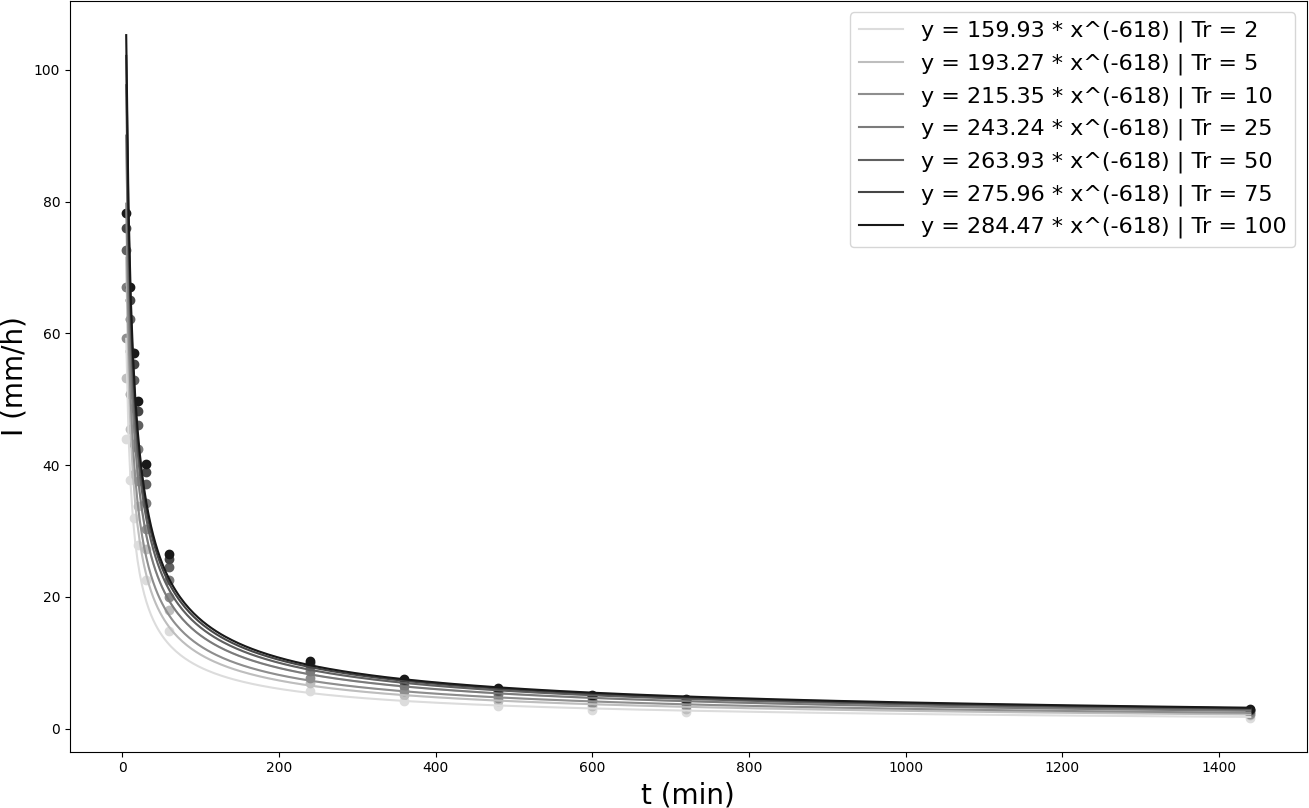
\includegraphics[width=.7325\linewidth]{figuras/apendice_curvas_idf_de_intensidade_e_duracao.png}
	\caption*{\textbf{Fonte:} De autoria própria (2023).}
	\label{fig:apendice_curvas_idf_de_intensidade_e_duracao.png}
\end{figure}

Tabela A.9 gerada a partir da Tabela A.6 e A.8, e das fórmulas (3.25) à (3.27):\bigskip

\begin{table}[ht]
\caption{Parâmetro \textit{c} de diferentes tempos de retorno}
\centering
\begin{tabular}{
>{\columncolor[HTML]{FFFFFF}}c 
>{\columncolor[HTML]{FFFFFF}}c 
>{\columncolor[HTML]{FFFFFF}}c 
>{\columncolor[HTML]{FFFFFF}}c 
>{\columncolor[HTML]{FFFFFF}}c 
>{\columncolor[HTML]{FFFFFF}}c 
>{\columncolor[HTML]{FFFFFF}}c 
>{\columncolor[HTML]{FFFFFF}}c }
\hline
Tr & $i_1$ & $t_1$ & $i_2$ & $t_2$ & $i_3$ & $t_3$ & $c_i$ \\ \hline
2 & 44.039 & 5 & 1.684 & 1440 & 8.612 & 113.314 & 4.235 \\
5 & 53.220 & 5 & 2.035 & 1440 & 10.407 & 113.314 & 4.235 \\
10 & 59.299 & 5 & 2.267 & 1440 & 11.596 & 113.316 & 4.236 \\
25 & 66.980 & 5 & 2.561 & 1440 & 13.097 & 113.314 & 4.235 \\
50 & 72.678 & 5 & 2.779 & 1440 & 14.212 & 113.312 & 4.235 \\
75 & 75.990 & 5 & 2.906 & 1440 & 14.859 & 113.314 & 4.235 \\
100 & 78.334 & 5 & 2.995 & 1440 & 15.318 & 113.313 & 4.235 \\ \hline
\end{tabular}
\caption*{\textbf{Fonte:} De autoria própria (2023).}
\end{table}

Parâmetro $c$ (A.24) da IDF, obtido a através da Tabela A.9 e da fórmula (3.28).\bigskip

\begin{equation}
c = \frac{29.645}{7} = 4.235
\end{equation}

\newpage

Ocorre então a soma do parâmetro $c$ (A.24) com as durações arbitradas como descrito no referencial teórico, para que assim se inicie o segundo uso do MMQ. Assim sendo, tem-se a Tabela A.10 gerada a partir da Tabela A.6 e das novas durações resultado da soma com o parâmetro $c$:\bigskip

\begin{table}[ht]
\caption{Duração mais parâmetro $c$ versus intensidades da chuva em mm/h}
\centering
\begin{tabular}{
>{\columncolor[HTML]{FFFFFF}}c 
>{\columncolor[HTML]{FFFFFF}}c 
>{\columncolor[HTML]{FFFFFF}}c 
>{\columncolor[HTML]{FFFFFF}}c 
>{\columncolor[HTML]{FFFFFF}}c 
>{\columncolor[HTML]{FFFFFF}}c 
>{\columncolor[HTML]{FFFFFF}}c 
>{\columncolor[HTML]{FFFFFF}}c }
\hline
\multicolumn{1}{c|}{\cellcolor[HTML]{FFFFFF}t + c} & \multicolumn{7}{c}{\cellcolor[HTML]{FFFFFF}I} \\ \cline{2-8} 
\multicolumn{1}{c|}{\cellcolor[HTML]{FFFFFF}(min)} & 2 anos & 5 anos & 10 anos & 25 anos & 50 anos & 75 anos & 100 anos \\ \hline
1444.235 & 1.684 & 2.035 & 2.267 & 2.561 & 2.779 & 2.906 & 2.995 \\
724.235 & 2.528 & 3.055 & 3.404 & 3.844 & 4.171 & 4.362 & 4.496 \\
604.235 & 2.908 & 3.514 & 3.916 & 4.423 & 4.799 & 5.018 & 5.173 \\
484.235 & 3.447 & 4.165 & 4.641 & 5.242 & 5.688 & 5.947 & 6.130 \\
364.235 & 4.278 & 5.170 & 5.760 & 6.506 & 7.060 & 7.382 & 7.609 \\
244.235 & 5.765 & 6.967 & 7.763 & 8.769 & 9.515 & 9.948 & 10.255 \\
64.235 & 14.891 & 17.995 & 20.051 & 22.648 & 24.575 & 25.694 & 26.487 \\
34.235 & 22.549 & 27.250 & 30.362 & 34.295 & 37.212 & 38.908 & 40.108 \\
24.235 & 27.959 & 33.788 & 37.647 & 42.523 & 46.141 & 48.243 & 49.731 \\
19.235 & 32.040 & 38.720 & 43.142 & 48.730 & 52.875 & 55.285 & 56.990 \\
14.235 & 37.681 & 45.537 & 50.738 & 57.309 & 62.185 & 65.018 & 67.024 \\
9.235 & 44.039 & 53.220 & 59.299 & 66.980 & 72.678 & 75.990 & 78.334 \\ \hline
\end{tabular}
\caption*{\textbf{Fonte:} De autoria própria (2023).}
\end{table}

Tabela A.11 gerada a partir da Tabela A.10, resultando nas variáveis que são usadas nas
fórmulas dos ajustes (3.22) e (3.23):\bigskip

\begin{table}[ht]
\caption{Variáveis usadas para o cálculo dos ajustes no segundo uso do MMQ.}
\centering
\begin{tabular}{
>{\columncolor[HTML]{FFFFFF}}c 
>{\columncolor[HTML]{FFFFFF}}c 
>{\columncolor[HTML]{FFFFFF}}c 
>{\columncolor[HTML]{FFFFFF}}c 
>{\columncolor[HTML]{FFFFFF}}c 
>{\columncolor[HTML]{FFFFFF}}c 
>{\columncolor[HTML]{FFFFFF}}c 
>{\columncolor[HTML]{FFFFFF}}c }
\hline
\multicolumn{1}{c|}{\cellcolor[HTML]{FFFFFF}log(t + c)} & \multicolumn{7}{c}{\cellcolor[HTML]{FFFFFF}log(I) = x} \\ \cline{2-8} 
\multicolumn{1}{c|}{\cellcolor[HTML]{FFFFFF}= y} & \multicolumn{1}{l}{\cellcolor[HTML]{FFFFFF}2 anos} & \multicolumn{1}{l}{\cellcolor[HTML]{FFFFFF}5 anos} & \multicolumn{1}{l}{\cellcolor[HTML]{FFFFFF}10 anos} & \multicolumn{1}{l}{\cellcolor[HTML]{FFFFFF}25 anos} & \multicolumn{1}{l}{\cellcolor[HTML]{FFFFFF}50 anos} & \multicolumn{1}{l}{\cellcolor[HTML]{FFFFFF}75 anos} & \multicolumn{1}{l}{\cellcolor[HTML]{FFFFFF}100 anos} \\ \hline
3.160 & 0.226 & 0.309 & 0.356 & 0.408 & 0.444 & 0.463 & 0.476 \\
2.860 & 0.403 & 0.485 & 0.532 & 0.585 & 0.620 & 0.640 & 0.653 \\
2.781 & 0.464 & 0.546 & 0.593 & 0.646 & 0.681 & 0.701 & 0.714 \\
2.685 & 0.537 & 0.620 & 0.667 & 0.719 & 0.755 & 0.774 & 0.787 \\
2.561 & 0.631 & 0.713 & 0.760 & 0.813 & 0.849 & 0.868 & 0.881 \\
2.388 & 0.761 & 0.843 & 0.890 & 0.943 & 0.978 & 0.998 & 1.011 \\
1.808 & 1.173 & 1.255 & 1.302 & 1.355 & 1.390 & 1.410 & 1.423 \\
1.534 & 1.353 & 1.435 & 1.482 & 1.535 & 1.571 & 1.590 & 1.603 \\
1.384 & 1.447 & 1.529 & 1.576 & 1.629 & 1.664 & 1.683 & 1.697 \\
1.284 & 1.506 & 1.588 & 1.635 & 1.688 & 1.723 & 1.743 & 1.756 \\
1.153 & 1.576 & 1.658 & 1.705 & 1.758 & 1.794 & 1.813 & 1.826 \\
0.965 & 1.644 & 1.726 & 1.773 & 1.826 & 1.861 & 1.881 & 1.894 \\ \hline
\end{tabular}
\caption*{\textbf{Fonte:} De autoria própria (2023).}
\end{table}

\newpage

Tabela A.12 gerada a partir da Tabela A.11, e das fórmulas dos ajustes (3.22), (3.23) e (3.24) usados na fórmula (3.20):\bigskip

\begin{table}[ht]
\caption{Ajustes do segundo uso do MMQ.}
\centering
\begin{tabular}{
>{\columncolor[HTML]{FFFFFF}}c 
>{\columncolor[HTML]{FFFFFF}}c 
>{\columncolor[HTML]{FFFFFF}}c 
>{\columncolor[HTML]{FFFFFF}}c 
>{\columncolor[HTML]{FFFFFF}}c 
>{\columncolor[HTML]{FFFFFF}}c 
>{\columncolor[HTML]{FFFFFF}}c 
>{\columncolor[HTML]{FFFFFF}}c }
\hline
Tr & $a_2$ & $a_1$ & $b_2$ & $b_1$ \\ \hline
2 & -0.677 & -0.677 & 2.362 & 230.03 \\
5 & -0.677 & -0.677 & 2.444 & 277.99 \\
10 & -0.677 & -0.677 & 2.491 & 309.74 \\
25 & -0.677 & -0.677 & 2.544 & 349.85 \\
50 & -0.677 & -0.677 & 2.579 & 379.62 \\
75 & -0.677 & -0.677 & 2.599 & 396.92 \\
100 & -0.677 & -0.677 & 2.612 & 409.16 \\ \hline
\end{tabular}
\caption*{\textbf{Fonte:} De autoria própria (2023).}
\end{table}

Gráfico de curvas na Figura A.2, que representa o da Figura 3.7 no referencial teórico,
gerado a partir da Tabela A.12 e da fórmula (3.20):\bigskip

\begin{figure}[!ht]
	\centering
	\caption{Relação entre intensidades e durações com complemento}
	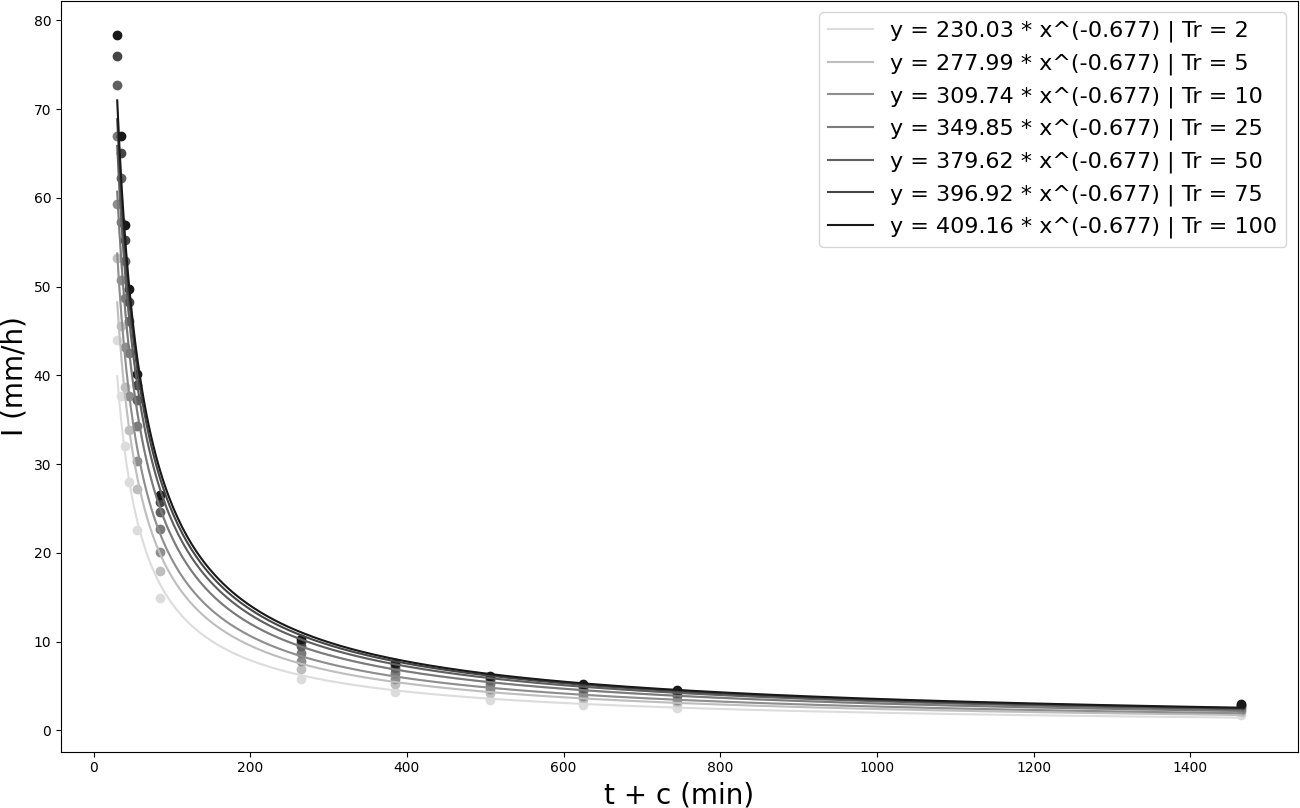
\includegraphics[width=.7525\linewidth]{figuras/apendice_curvas_idf_de_intensidade_e_duracao_com_complemento.png}
	\caption*{\textbf{Fonte:} De autoria própria (2023).}
	\label{fig:apendice_curvas_idf_de_intensidade_e_duracao_com_complemento.png}
\end{figure}

O parâmetro $d$ (A.25) da IDF é obtido a através da Tabela A.12, e da fórmula (3.29).\bigskip

\begin{equation}
d = -1 * \frac{- 4.739}{7} = 0.677
\end{equation}\bigskip

Chegando ao fim do cálculo, o terceiro uso do MMQ será iniciado, porém agora para funções de ajuste linear. Assim sendo, tem-se a Tabela A.13 gerada a partir da Tabela A.12, resultando nas variáveis que são usadas nas fórmulas dos ajustes (3.22) e (3.23):

\newpage

\begin{table}[ht]
\caption{Variáveis usadas para o cálculo dos ajustes no terceiro uso do MMQ.}
\centering
\begin{tabular}{
>{\columncolor[HTML]{FFFFFF}}c 
>{\columncolor[HTML]{FFFFFF}}c }
\hline
log(Tr) & $b_2$ \\
= y & = x \\ \hline
2.000 & 2.612 \\
1.875 & 2.599 \\
1.699 & 2.579 \\
1.398 & 2.544 \\
1.000 & 2.491 \\
0.699 & 2.444 \\
0.301 & 2.362 \\ \hline
\end{tabular}
\caption*{\textbf{Fonte:} De autoria própria (2023).}
\end{table}

Ajustes lineares (A.26) e (A.27) do terceiro uso do MMQ, a partir dos dados da Tabela A.13 aplicados às fórmulas (3.22), (3.23) e (3.30):\bigskip

\begin{equation}
a_1 = a_2 = 0.143
\end{equation}

\begin{equation}
b_1 = 10^{b_2} = 10^{2.336} = 216.674
\end{equation}\bigskip

Gráfico de linear na Figura A.3, que representa o da Figura 3.8 no referencial teórico,
gerado a partir da Tabela A.13 e da fórmula (3.21):\bigskip

\begin{figure}[!ht]
	\centering
	\caption{Relação entre tempos de retorno e ajustes}
	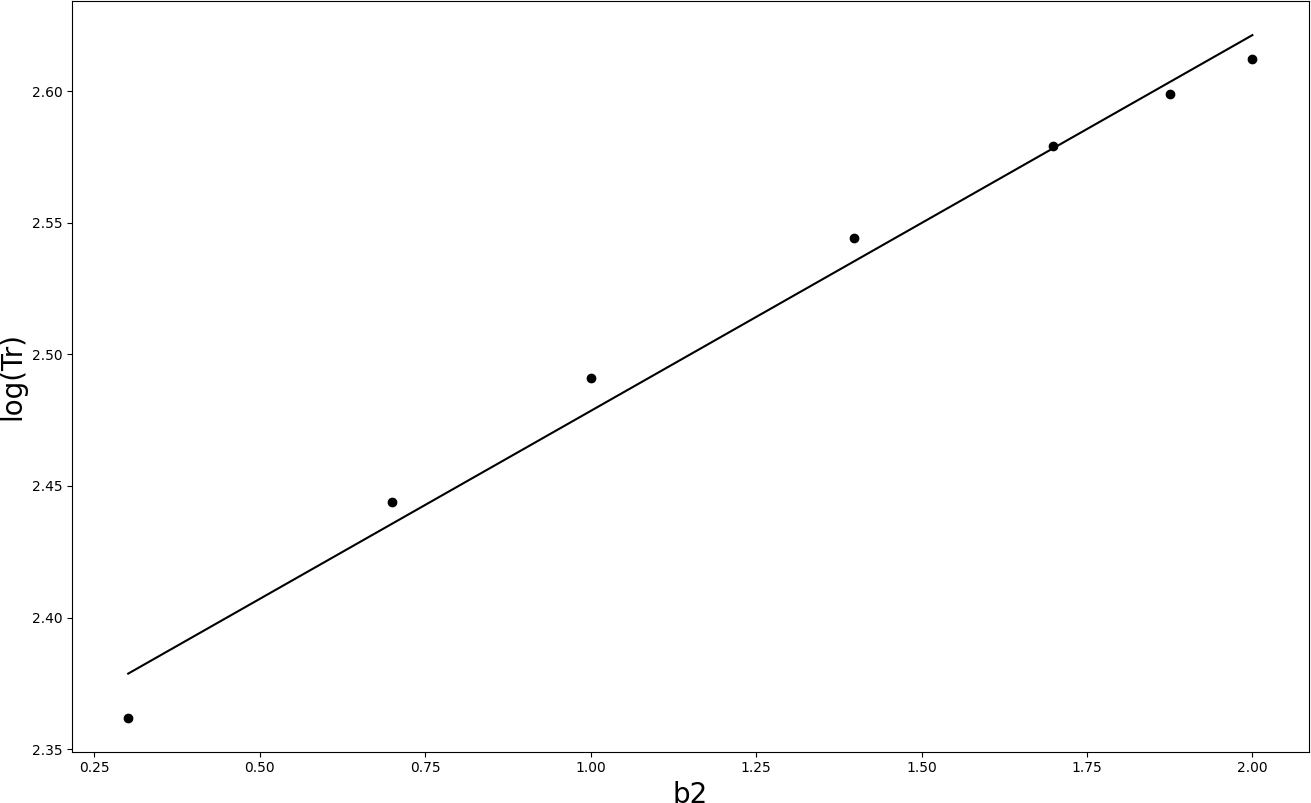
\includegraphics[width=.7325\linewidth]{figuras/apendice_reta_de_tempo_de_retorno.png}
	\caption*{\textbf{Fonte:} De autoria própria (2023).}
	\label{fig:apendice_reta_de_tempo_de_retorno.png}
\end{figure}

\newpage

Parâmetros $a$ (A.28) e $b$ (A.29) da IDF obtidos através das fórmulas (3.31) e (3.32) sucessivamente.\bigskip

\begin{equation}
a = b_1 = 216.674
\end{equation}

\begin{equation}
b = a_1 = 0.143
\end{equation}\bigskip

Assim sendo, é possível gerar a IDF a partir da fórmula (3.1) e dos resultados (A.24), (A.25), (A.28) e (A.29):\bigskip

\begin{equation}
I = \frac{216.743 * Tr^{0.143}}{(t + 4.235)^{0.677}}
\end{equation}\bigskip

E então, chega-se ao resultado final que é a equação para o local qual os dados foram coletados.\bigskip\bigskip

\addcontentsline{toc}{chapter}{APÊNDICE B}

\begin{center}
\noindent\textbf{APÊNDICE B}
\end{center}

O documento que segue a partir da próxima lauda trata-se do manual de uso prático da ferramenta computacional \textbf{Intensio}, elaborado para auxilio ao usuário da mesma como explicado anteriormente no presente trabalho.

% Manual de Uso

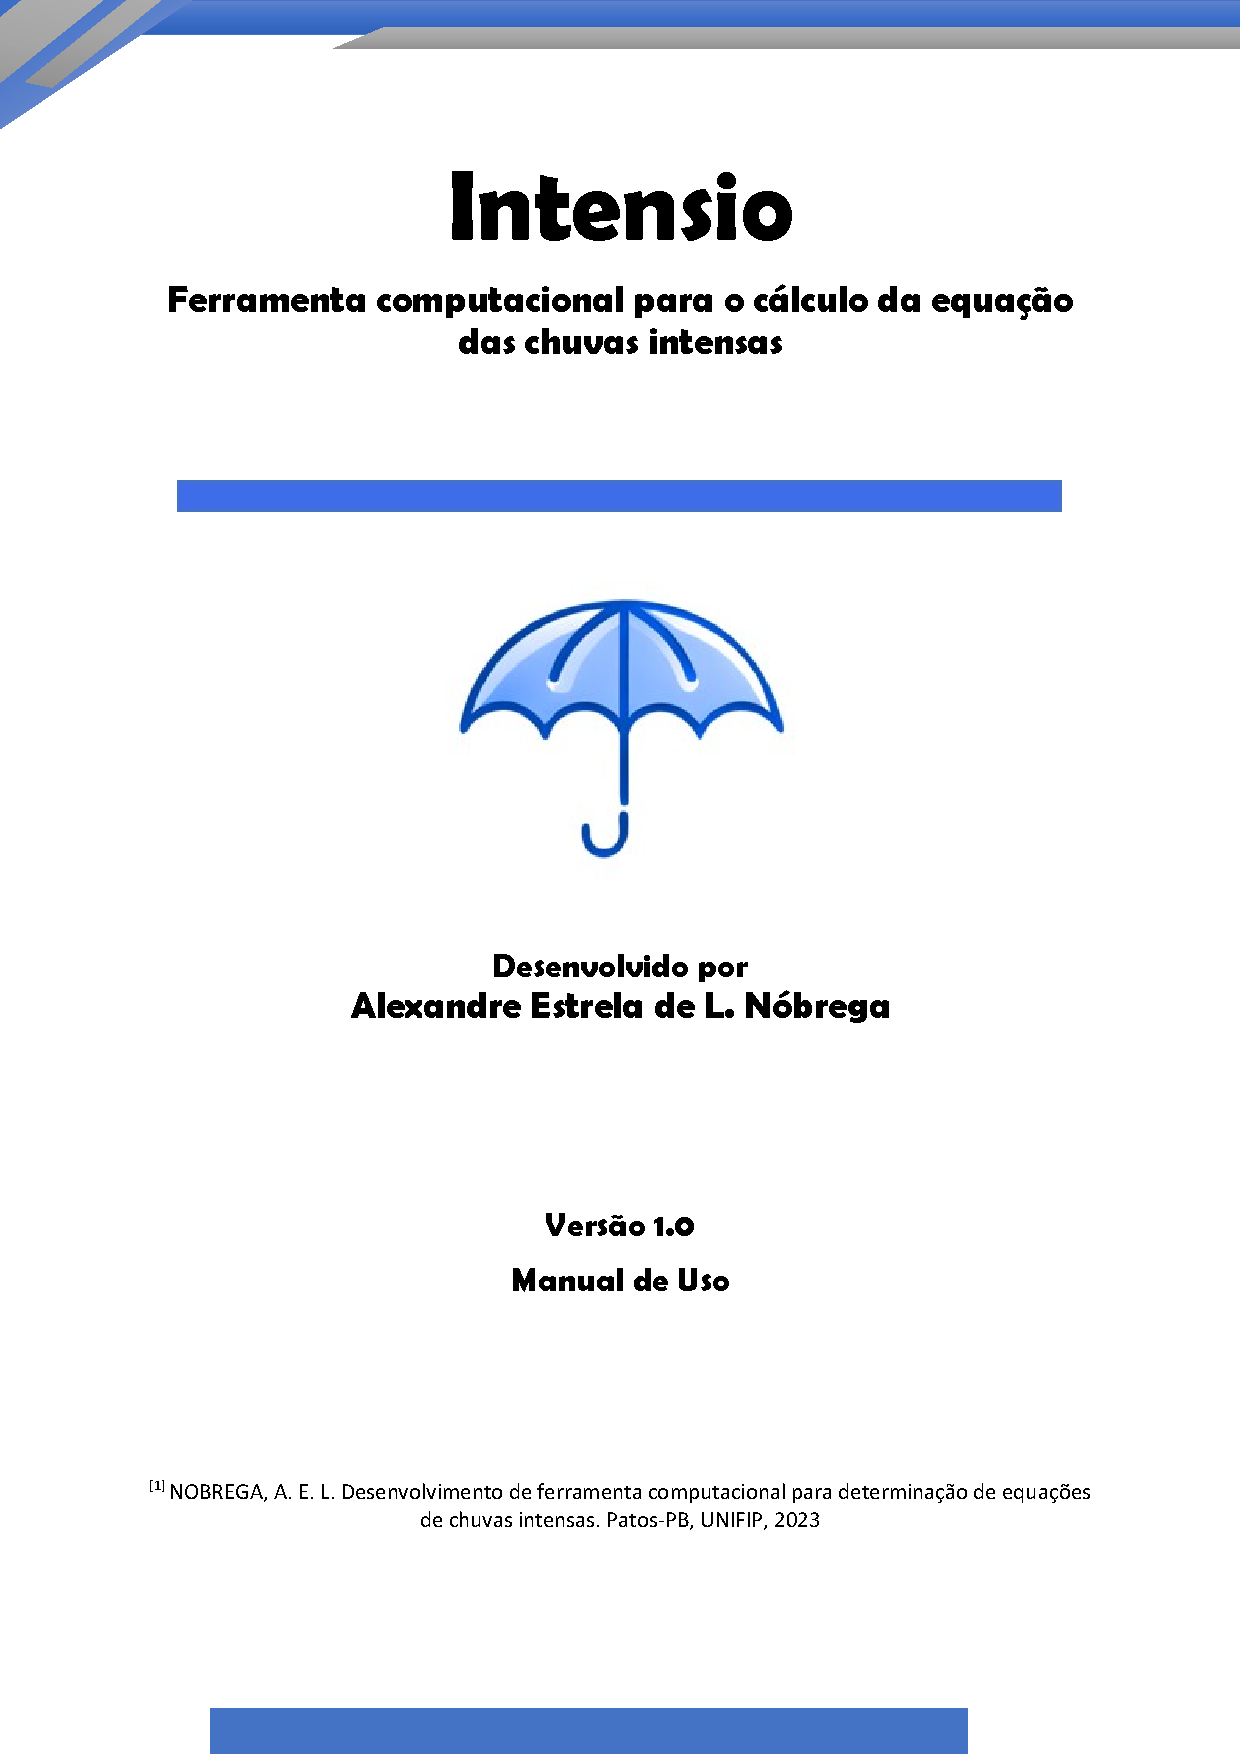
\includepdf[pages=-]{documentos/manual_de_uso.pdf}